\documentclass[usenames, dvipsnames, t]{beamer}

%\usepackage{geometry}
%\geometry{legalpaper, textwidth=426pt}
%\usepackage[T1]{fontenc}
%\usepackage{fourier}
\usepackage{graphicx}
%\graphicspath{{Figures/}}
%
\usepackage[english]{babel}															% English language/hyphenation
%\usepackage[protrusion=true,expansion=true]{microtype}
\usepackage{amsmath,amsfonts,amsthm} % Math packages
\usefonttheme[onlymath]{serif}
\usepackage{graphicx, adjustbox}
\graphicspath{{figures/}}
%\usepackage{url}
\newcommand{\red}[1]{\textcolor{red}{#1}}
%
%% Self included packages
%%\usepackage[labelfont=sf,			hypcap=false,			format=hang,			width=\columnwidth]{caption}
%\usepackage{amsmath}
%\usepackage{wrapfig}
\usepackage[ruled, vlined]{algorithm2e}
\usepackage{pgfplots}
%\pgfplotsset{soldot/.style={color=blue,only marks,mark=*}} \pgfplotsset{holdot/.style={color=blue,fill=white,only marks,mark=*}}
\pgfplotsset{compat=1.12}
\usepackage{xcolor}
\usepackage{tikz}
\usetikzlibrary{graphs, graphs.standard, shapes.misc, positioning, fit, shadows, calc, snakes, shapes, patterns, arrows.meta, matrix, shapes.geometric}
% \usepackage[noend]{algpseudocode}
\usepackage{hyperref}
\hypersetup{
    colorlinks,
    citecolor=black,
    filecolor=black,
    linkcolor=black,
    urlcolor=black
}
%\usepackage{ifthen}
\usepackage{bm}
%\usepackage{enumerate}
%%%%%%%%%%%%%%%%%%%%%%%%%%%%%%%%%%%%%%%%%%%%%%%%%%%%%%%%%%%%%%%%%%%%%%%%%%%
\usetheme{CambridgeUS}
\usecolortheme{beaver}
\usepackage[english]{babel}

\setbeamertemplate{section in toc}{\inserttocsection}
\setbeamertemplate{subsection in toc}{\hspace{1.2em}~\inserttocsubsection\par}

\setbeamerfont{section in toc}{size=\small}
\setbeamerfont{subsection in toc}{size=\footnotesize}

\setbeamertemplate{itemize item}{\color{red}$\circ$}
\setbeamertemplate{itemize subitem}{\color{red}$\circ$}

\setbeamertemplate{enumerate item}[default]
\setbeamercolor*{enumerate item}{fg=red}
\setbeamercolor*{enumerate subitem}{fg=red}
\setbeamercolor*{enumerate subsubitem}{fg=red}

\setbeamertemplate{footline}
{
  \leavevmode%
  \hbox{%
  \begin{beamercolorbox}[wd=.2\paperwidth,ht=2.25ex,dp=1ex,center]{author in head/foot}%
  	\usebeamerfont{author in head/foot}\insertshortauthor
  \end{beamercolorbox}%

  \begin{beamercolorbox}[wd=.5\paperwidth,ht=2.25ex,dp=1ex,center]{title in head/foot}%
    	\usebeamerfont{title in head/foot}\insertshorttitle\hspace*{3em}
  \end{beamercolorbox}%

  \begin{beamercolorbox}[wd=.3\paperwidth,ht=2.25ex,dp=1ex,right]{date in head/foot}%
    	\usebeamerfont{date in head/foot}\insertshortdate{}\hspace*{2em}
	\insertframenumber{} / \inserttotalframenumber\hspace*{2ex}
  \end{beamercolorbox}}%
  \vskip0pt%
}

\title{DiffSim 24.02.}
\subtitle{}
\author{Ludwig Winkler}
\institute{Machine Learning Group \\ TU Berlin}
\date{\today}


%%%%%%%%%%%%%%%%%%%%%%%%%%%%%%%%%%%%%%%%%%%%%%%%%%%%%%%%%%%%%%%%%%%%%%%%%%%%
\begin{document}

\def\mathn#1{\mathnormal{#1}}
\def\thet{\bm{\theta}}
\def\V{\mathn{V}}
\def\Q{\mathn{Q}}
\def\R{\mathn{R}}
\def\r{\mathn{r}}
\def\G{\mathn{G}}
\def\n{\mathn{n}}
\def\A{\mathn{A}}
\def\T{\mathn{T}}
\def\W{\mathn{W}}
% \def\E{\mathbb{E}}

\def\w{\mathn{w}}
\def\p{\mathn{p}}
\def\q{\mathn{q}}
\def\a{\mathn{a}}
\def\r{\mathn{r}}
\def\s{\mathn{s}}
\def\t{\mathn{t}}
\def\dist{1}

\newcommand{\E}{\mathbb{E}}

\tikzset{ shorten <>/.style={ shorten >=#1, shorten <=#1 } }


\begin{frame}
	\titlepage
\end{frame}

% \begin{frame}
% \frametitle{Outline}
% \tableofcontents
% \end{frame}

\begin{frame}
	\frametitle{DiffSim - Idea}
	\begin{itemize}
		\item Autodiff frameworks work great for machine learning: we compute gradients for parameters conveniently
		\item Why stop at computing parameter gradients? Why not autodiff arbitrary code?
		\item Big part of modern engineering/research are based on computer models/simulations
		\item[]
		\item Let's autodiff entire computer models/simulations!
		\item Question: What could we do with that?
	\end{itemize}
\end{frame}

\begin{frame}
	\frametitle{What's happened so far}
	\begin{itemize}
		\item Simulation of explicit high-dim simulation vs low-dim latent simulation [Rotating Gaussian distribution]
		\item Parts of latent simulation is done by neural network ODE
		\item[] 
		\item Chaotic system with external force field [Double Pendulum]
		\item[] 
		\item Three Body Problem of rotating planets [N-Body Problem]
	\end{itemize}
\end{frame}

\begin{frame}
	\frametitle{What's to discuss}
	\framesubtitle{Problem of the day ... and months :( }
	\begin{itemize}
		\item Ultimately we're training on a regression problem
		\item Long integration horizons aggravate basically tiny error
		\item Neural networks hide a lot of possibly random behaviour in their weights in unknown data regions
		\item[] 
		\item Personal opinion: NN's bad for long term simulations (if we have the precise simulation)
		\item Classification doesn't care if it's 0.9 or 0.901, as it only wants the maximum
	\end{itemize}
\end{frame}

\begin{frame}
	\frametitle{What's to discuss}
	\framesubtitle{Pivot Idea (and maybe what you wanted all along)}
	\begin{itemize}
		\item Brenner AutoDiff Optimal Control paper
		\begin{itemize}
			\item ML control on 2D Ising lattice model
			\item ML control interacts in discreet way with simulation
			\item ML control basically classification not regression
		\end{itemize}
		\item[]
		\item Simulations offer precise computations (so let them do the heavy work)
		\item Autodiff through simulations to train hyperparameters of simulation
	\end{itemize}
\end{frame}

\begin{frame}
	\frametitle{What's to discuss}
	\framesubtitle{Hyperparameter Optimization of Double Pendulum Simulation}
	\begin{itemize}
		\item Masses of joints (m1, m2) and gravitational constant g learned via DiffSim for Double Pendulum
	\end{itemize}
	\centering
	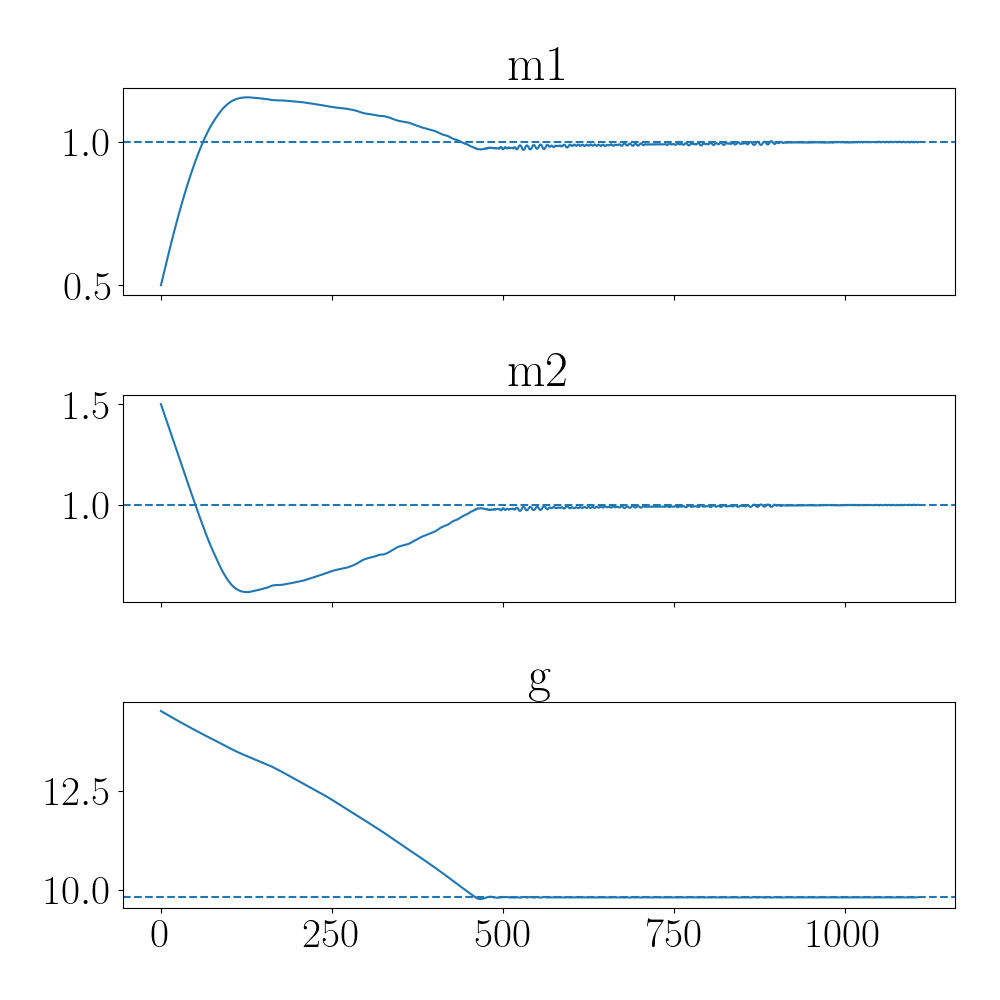
\includegraphics[height=0.7\textheight]{myplot.png}
\end{frame}

\begin{frame}
	\frametitle{What's to discuss}
	\framesubtitle{Pivot Idea (and maybe what you wanted all along)}
	\begin{itemize}
		\item ML models trained via Reverse Mode AutoDiff
		\item Forward Mode AutoDiff allows differentiation of arbitrarily long simulations
		\item Simulation classes that could be tested out?
	\end{itemize}
\end{frame}

\begin{frame}
	\frametitle{Next Step}
	\begin{itemize}
		\item Require Forward Mode AutoDiff (ForAD) for simulations
		\item ForAD is memory independent
		\item Just keeps on multiplying memory constant Jacobians during simulation
		\item JAX and recently PyTorch offer ForAD
		\item[] 
		\item Train on masses in planetary n-body problem via gradient training
	\end{itemize}
\end{frame}




\end{document}
